In this section we will mention our final model and its performance, we have three combinations we will illustrate.

\begin{enumerate}
	\item CNN.
	\item HOG and Landmarks.
	\item CNN with HOG and Landmarks.
\end{enumerate}
See figure \ref{cnn_lm_hog} for full model architecture.
\begin{figure}
	\centering
	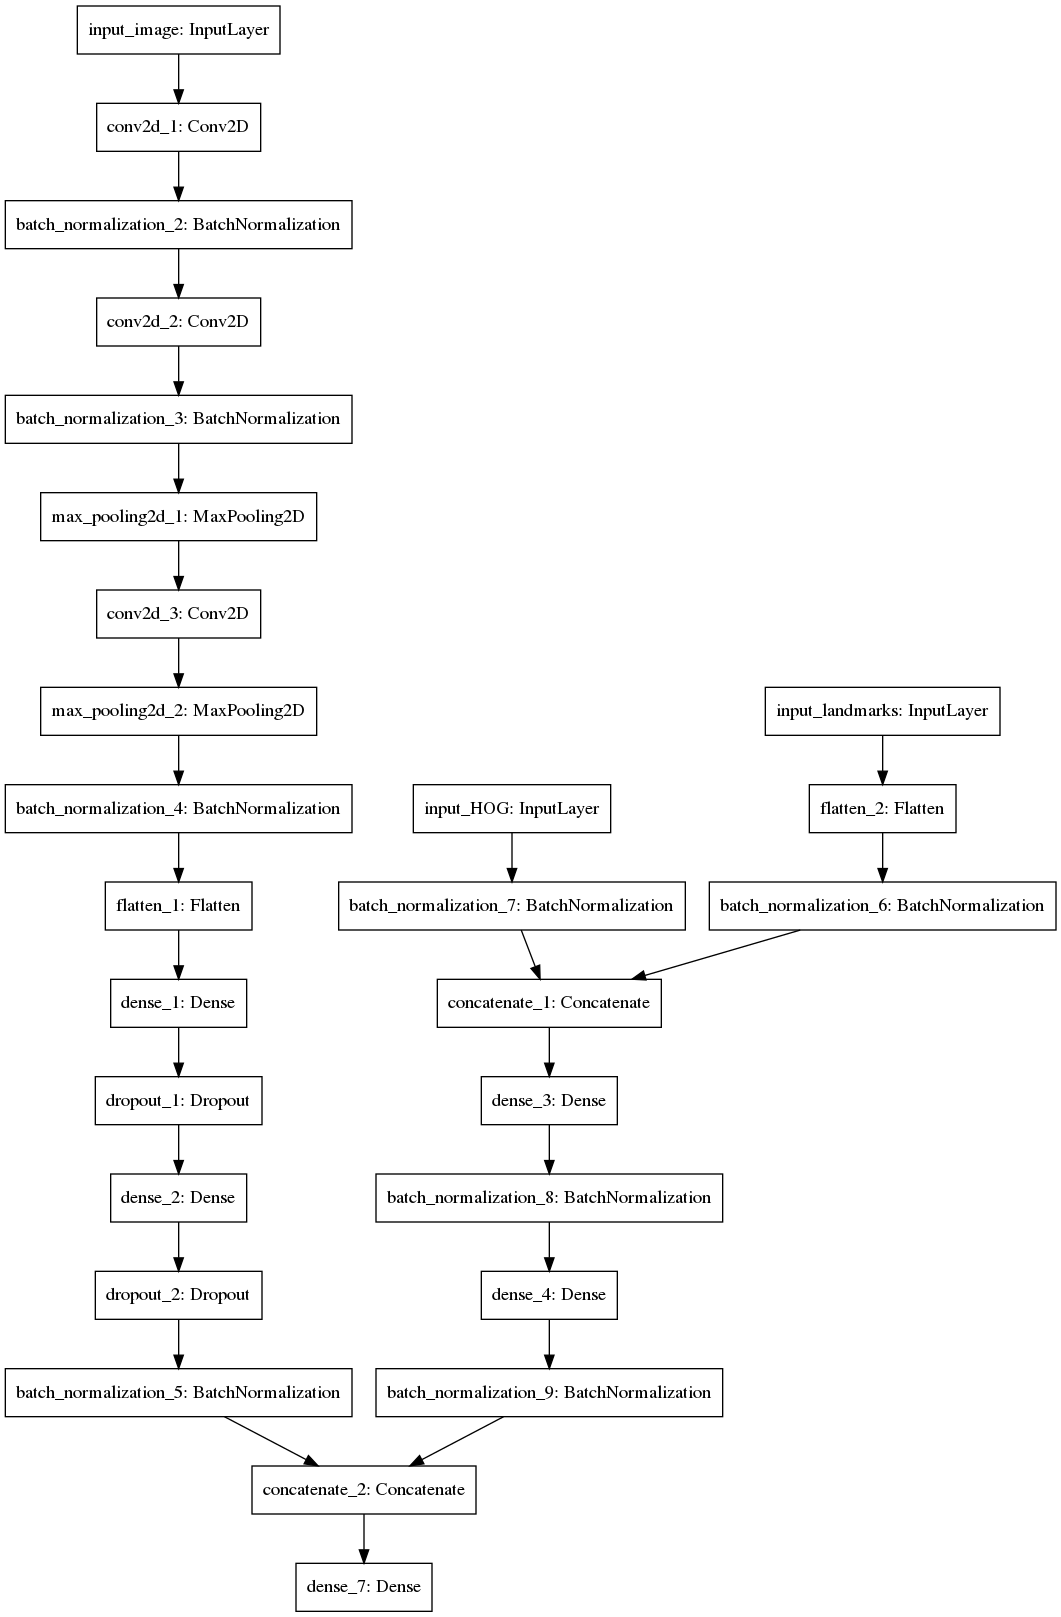
\includegraphics[width=1\textwidth]{images/cnn_hog_lm.png}
	\caption{Diagram of CNN + HOG + LM structure}
	\label{cnn_lm_hog}
\end{figure}

Note that the model is configured in such a way that we can enable/disable any of the 3 paths (CNN, HOG, LM) easily, we finally choose the model with only Landmarks and HOG paths with final testing accuracy of 98\% on the combination of CK+ and RafD datasets.
\newline
For the working model as we noticed that :
\begin{enumerate}
	\item Using landmarks and hog as a feature extraction then feed it to model layers gives a good accuracy with small model size (1M) and the training process itself is too fast compared to CNN.
	\item Using only CNN works well giving the same accuracy, but the model size is large and takes to much time for training.
	\item On combining CNN with landmarks and HOG , we do not notice any change in accuracy as CNN itself does feature extraction, so adding them together only makes training process harder and longer, it also makes the final model larger with no effect on accuracy.
\end{enumerate} 